\chapter{KOORDINAT}

Koordinat atau alamat keberadaan/posisi suatu wilayah dijabarkan ke dalam angka. Koordinat yang sering digunakan ada 2 (dua) jenis, yaitu koordinat geografi dan koordinat UTM (Universal Transversal Mercator).

\begin{itemize}
  \item Contoh koordinat Geografi
  
  X = $108^{\circ}30'50"; Y=7^{\circ}30'50"$
  
  \item Contoh Koordinat UTM
  
  X = 480000; Y=9800000
\end{itemize}

Datum titik nadir (konstanta/ketetapan), bumi bentuknya bulat sedangkan derajat/geografi di jabarkan di bidang datar dengan dibuat grid dan diberikan nomor. Tahun survey terbaru adalah tahun 1984 sehingga dikenal dengan \textbf{WGS1984}.

Pemilihan proyeksi \textbf{WGS1984} dilakukan dengan memilih menu Map -\textgreater Options, sehingga akan muncul jendela berikut :

\begin{figure}[H]
  \centering
  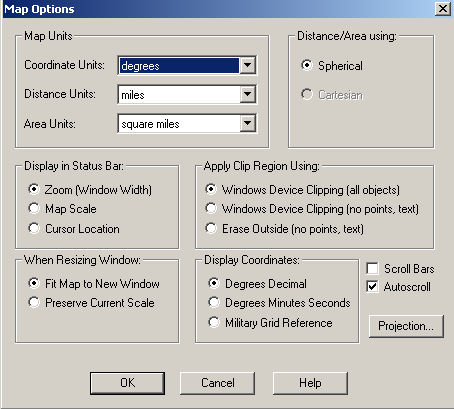
\includegraphics[width=1\textwidth]{./resources/045-jendela-map-option}
  \caption{Jendela Map Options}
\end{figure}

Kemudian klik \textbf{Projection}, sehingga muncul jendela \textit{projection} seperti berikut :

\begin{figure}[H]
  \centering
  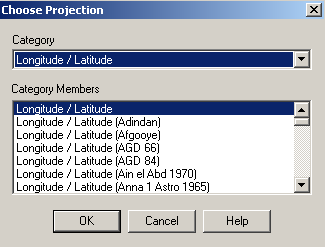
\includegraphics[width=1\textwidth]{./resources/046-jendela-projection}
  \caption{Jendela Projection}
\end{figure}

Terakhir memilih Kategori \textbf{Universal Transverse Mercator (WGS 84)}, kemudian memilih UTM Zone 49 pada Category Members dan menekan tombol \textbf{OK}, karena posisi Kabupaten Brebes berada pada Zona 49 UTM/WGS84, seperti gambar berikut :

\begin{figure}[H]
  \centering
  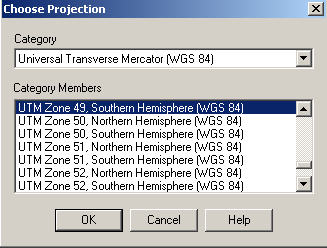
\includegraphics[width=1\textwidth]{./resources/047-pemilihan-utm-wgs84}
  \caption{Pemilihan UTM WGS 84 Zona 49 S}
\end{figure}